\documentclass{article}
\usepackage{amsmath,amsthm,amssymb}
\usepackage{graphicx}
\usepackage{float}
\usepackage{booktabs}
\usepackage[style=authoryear-ibid,backend=biber]{biblatex}
\title{Structural Differences Between Random Graphs and Small World, Scale-Free Graphs }
\date{08/02/2023}
\author{Thomas Draycott}
\addbibresource{references.bib}
\graphicspath{ {./images/} }
\begin{document}
    \maketitle
    \pagenumbering{arabic}
    \newpage
    \begin{abstract}
        TO DO LAST
    \end{abstract}
    \tableofcontents
    \newpage
    \section{Introduction}
    This project investigates the structural differences between random graphs and small-world, scale-free graphs and in particular, Barabási-Albert graphs.\\
    Later, we will use an SIRD model as a vehicle to explore whether these structural differences can affect a random process. Traditionally a project that contains an SIRD model would focus on the model as its core concept. Alternatively we will only use it as a simple lens to investigate the differences between graph structures. Therefore, little time will be afforded to the mathematics behind the SIRD simulation, more time will be afforded to how it computes on our graphs.\\
    Random graphs were chosen as the comparison because they are random they are free of overarching structures that are present in other types of graph.\\
    The motivation for this project stems from my deep interest in graph theory. Additionally, with the recent COVID-19 pandemic I wanted to explore if it is how the way populations are internally structured which lead to a significant difference in the spread of disease.\\
    Code and data used can be found at the following link:\\ 
    https://www.dropbox.com/sh/ilb1vjvloguj33l/AAA2jwv5oi5SeFTtlSgjPn3Fa?dl=0
    \section{Literature Review}
        \subsection{Graph Theory}
        Graph Theory is the study of networks where vertices are connected by edges (The words 'node' and 'vertex' will be used interchangeably as will 'network' and graph however graph will be used for more abstract representations). A simple graph contains no self loops and there can only be one edge between each pair of nodes. We will only be focusing on simple undirected graphs in this project and any graph mentioned can be assumed to be simple and undirected. A strict definition of simple graphs is as follows: Let $G$ be a graph, $G$ is an ordered pair $G=(V,E)$ comprising $V$: a set of vertices and $E\subseteq \{\{x,y\} | x,y \in V \text{ and } x\neq y\}$: a set of edges which are unordered pairs of vertices \parencite{bender2010lists}.
        \subsection{Random Graphs}
        In 1959, Paul Erd\"{o}s and Alfr\'{e}d R\'{e}nyi published their paper 'On Random Graphs' \parencite{erd6s1959random}. Independently, Edgar Nelson Gilbert published his paper 'Random Graphs' \parencite{gilbert1959random}. Both papers describe how to create a graph using probabilities which became a very useful tool for solving problems in graph theory. In particular, problems in which they aimed to prove the existence of certain graphs held various properties or to provide a strong definition for what it meant for a property to hold for almost all graphs.\\ 
        However, Erd\"{o}s' and Gilbert's models differed in how they worked. The Erd\"{o}s-R\'{e}yi model works as follows; to generate a random graph $G(N,M)$ where $N$ is the number of nodes in the graph and $M$ is the total number of edges to be added, randomly pick $M$ pairs of vertices from the set of all combinations of two vertices, ignoring repeats and draws edges between them. In this model the average degree is easily calculated. However, it is rare that the number of edges will be exact which brings on to the Gilbert model. For the Gilbert Model we define the random graph $G$ as such; $G(N,p)$ where $N$ is the total number of nodes and $p$ is the probability of joining two vertices together and works as follows: draw $N$ nodes for the graph, select a vertex pair, generate a random number between $0$ and $1$, if the number exceeds $p$ draw en edge between those two vertices, repeat for all vertex pairs once. For the rest of this paper we will use 'random graph' to refer to Gilbert model random graphs as they better represent real networks because the number of edges is not fixed. 
        \subsection{Small World Graphs}
        In May 1967,the Professor of Psychology at the Graduate School and University Center of the City University of New York, Stanley Milgram ran an experiment to see if a person living
        in Omaha, Nebraska could send a parcel to a stockbroker in Boston, Massachusetts that they had never met personally by asking the subjects to give the parcel to someone they thought may know the recipient \parencite{milgram1967small}. In his experiment he found the average path length to reach the stockbroker was 5.5, which created the term
        six degrees of separation. However, Milgram's experiment had flaws which puts the exact number into doubt. This idea of having such a small average path length for a numerous amount of nodes the hallmark of a small world graph.\\
        A Small world graph is formally defined by the following property: $L\propto\log{N}$ where $L$ is the average shortest path length of the network and $N$ is the total number of nodes \parencite{Watts1998}. Several models exist to generate small world graphs such as the Watts-Strogatz Model.

        \subsection{Scale Free Graphs}
        In networks that appear in the real world such as the internet and social groups, there exist nodes known as "hubs"  (nodes that have a significantly higher degrees than the average of the graph). This is an important property encapsulated in Scale-Free Graphs.\\ 
        Scale-free Graphs are formally defined by the following power law: $P(k) \sim  k^{-\gamma }$, $k$ is the degree of a vertex, $P(k)$ is the probability of a node having degree $k$ and $\gamma$ is a parameter determined by the graph typically $2<\gamma<3$ \parencite{onnela2007structure}.

        \subsection{Barabasi-Albert Model}
        In 1999, Albert-László Barabási and Réka Albert developed the Barabási-Albert Model which generates small world, scale free graphs by a process of preferential attachment \parencite{barabasi1999emergence}. The model works as such: define two parameters $N$ (The number nodes the graph at the end of the process will have) and $e$ (the number of edges added for each new node) take a seed graph (A graph we start with originally that the model will grow from), add one new node to the graph, using preferential attachment add $e$ edges from the new node to nodes on the seed graph (With no loops or self loops), continue until there are $N$ nodes on the graph.\\
        'Preferential attachment' describes a 'rich get richer effect' that means the higher the degree of the node the more likely it will gain a new edge. This is described by the following formula $\prod (k_{i}) = \frac{k_{i}}{\sum_{\forall j} {k_{j}}}$ where $k_{i}$ is the degree of node $i$. 
        \subsection{SIRD Model}
        SIRD stands for Susceptible, Infected, Recovered and Dead which are the four states each individual in the model can take. There are many ways of implementing a model like this such as a virus having specific infection 'power' and mortality rates or having the infection be determined entirely by the individual. SIRD models vary massively in the assumptions they make, we will be assuming a discrete SIRD model with a constant infection rate, constant recovery rate and total immunity after a node has been infected once.    \section{Mathematical Methods}
        \subsection{Graph Theory}
            \subsubsection{Degrees}
            We will provide some key definitions and results from Graph Theory which will be useful for the further topics \parencite{barabasi2013network}.\\
            Degree: The number of edges attached to a node (Commonly written as $k_i$ denoting the degree $k$ of node $i$).\\ 
            We can calculate the number of edges $L$ of a graph from the sum of the degrees that is: 
            \begin{align*}
                L=\frac{1}{2}\sum_{i=1}^{N} k_{i}
            \end{align*}
            Average degree:
            \begin{align*}
                \langle k \rangle = \frac{1}{N} \sum_{i=1}^{N}k_{i} = \frac{2L}{N}
            \end{align*}
            ($\langle k \rangle$ and $\overline{k}$ will be used interchangeably, but $\langle k \rangle$ will be more common)
            Degree distribution: The probability distribution of the degrees of the graph will be very relevant in the later sections, so we will define it here as $p_k$ which is the probability a node has degree $k$.
            \begin{align*}
                &\text{As $p_k$ is a probability we must normalize it with the following condition:}\\
                &\sum_{k=1}^{\infty}p_{k} = 1\\
                &\text{For a network with $N$ nodes where $N_k$ is the number of nodes with degree $k$}\\
                &p_{k} = \frac{N_k}{N}\\
                &\text{With this we can redefine $\langle k \rangle$ as:}\\
                &\langle k \rangle = \sum_{k=0}^{\infty}kp_{k}
            \end{align*}
        \subsubsection{Adjacency Matrix}
            Graphs can also be represented by adjacency matrices. We define the matrix $A$, entry $A_{i,j} = 1$ if there is an edge between node $i$ and node $j$ else $A_{i,j} = 0$. For an undirected graph $A$ is symmetrical.\\
        \subsubsection{$L_{\text{max}}$}
            The total number of edges $L$ for a graph is bounded by $L_{\text{max}}$ and $L=0$
            \begin{align*}
                L_{\text{max}} =  \frac{N(N-1)}{2}\\
            \end{align*}
            We can see this by the most edges a simple graph can have is if it is a complete graph and complete graphs have $\frac{N(N-1)}{2}$ therefore a non-complete graph must have fewer edges.\\
            Most real networks are sparse that is $L\ll L_{\text{max}}$\\
        \subsubsection{Paths}
        A path is an ordered list of nodes describing a walk from each node to another. A Path length is the number of nodes contained in a path. The shortest path is the path between node $i$ and node $j$ with the smallest possible path length and is usually denoted as $d_{i,j}$ or just $d$. The diameter of a graph is defined as the longest shortest path of a graph and is denoted as $d_{\text{max}}$.\\
        The average shortest path length is defined as the average of the shortest paths between all pairs of nodes and is denoted as $\langle d \rangle$ and is calculated as such:
        \begin{align*}
            &\langle d \rangle = \frac{1}{N(N-1)}\sum_{i,j=1,N | i\neq j}d_{i,j}
        \end{align*}

        \subsubsection{Clustering Coefficient}
        The local clustering coefficient, as defined by \parencite{Watts1998}, measures the extent to which a node's neighbors connect with one another. \parencite{barabasi2013network} explains that this coefficient is calculated for a node $i$ based on its degree, denoted as $k_i$
            \begin{align*}
                &C_{i} = \frac{2L_{i}}{k_{i}(k_{i}-1)}\\
                &\text{Where $L_{i}$ is the number of links between the $k_i$ neighbours of node $i$. $C_{i}$ is between $0$ and $1$}
            \end{align*}
            $C_i$ represents the proportion that the neighbours of node $i$ are connected\\
            We can define the average clustering coefficient of a graph as such:
            \begin{align*}
                \langle C \rangle = \frac{1}{N}\sum_{i=1}^{N}C_{i}
            \end{align*}
            $\langle C \rangle$ can also be interpreted as the probability two neighbours of a randomly selected node link to each other
        \subsubsection{Global Cluserting Coefficient}
        The Global Clustering Coefficient is another measure of a graph's clustering. It is defined as such:
        \begin{align*}
            &\text{Let $L_\triangle$ be the number of closed triangles in the graph}\\
            &\text{Let $L_t$ the number of connected triplets}\\
            &C_g = \frac{3L_\triangle}{L_t}
        \end{align*}
        Note the average clustering coefficient and global clustering coefficient are not equal. Although it is a useful measure the literature focuses more on the average clustering coefficent, so that will be used for the rest of the project.

        \subsection{Random Graphs}
        For a random graph $G(N,p)$ we will define some key behaviours and values.
            \subsubsection{Number of Edges}
            We can begin by defining the probability of a random graph having exactly $L$ edges:
            To begin, there are $\frac{N(N-1)}{2}$ pairs of nodes that can potentially be connected with edges. The probability that $L$ out of these pairs have successfully formed an edge is $p^L$, while the probability that the remaining $\frac{N(N-1)}{2} - L$ pairs have not formed an edge is $(1-p)^{\frac{N(N-1)}{2} - L}$. Ultimately, there are $\binom{\frac{N(N-1)}{2}}{L}$ ways to connect $L$ edges among the $\frac{N(N-1)}{2}$ pairs of nodes. Taking the product of these factors we gain:
            \begin{align*}
                p_{L} = \binom{\frac{N(N-1)}{2}}{L}p^L(1-p)^{\frac{N(N-1)}{2} -L}
            \end{align*}
            Which is clearly a binomial distribution, therefore the mean number of edges $\langle L \rangle$ is given by $np$ which for this example is equal to $p\frac{N(N-1)}{2}$. We also obtain the average degree of the random graph:
            \begin{align*}
                \langle k \rangle = \frac{2 \langle L \rangle}{N} = p(N-1)
            \end{align*}
            Note that $N-1$ is the maximum degree a node can have in this graph.
            \subsubsection{Degree distribution}
            Similarly to the case of edges above, we can construct a binomial distribution for the degrees of the random graph. The probability a randomly chosen node will have degree $k$ will be a product of three terms defined as follows: The probability the node has $k$ edges is $p^k$, the probability the remaining $N-1-k$ edges are missing is $(1-p)^{N-1-k}$. The number of ways a node can have degree $k$ from degree $N-1$ is $\binom{N-1}{k}$ thus.
            \begin{align*}
                p_{k} = \binom{N-1}{k}p^k(1-p)^{N-1-k}
            \end{align*}  
            Using the properties of the binomial distribution we see that the average degree is $p(N-1)$ and the variance is $p(N-1)(1-p)$
            \subsubsection{The Poisson Approximation}
            Most real networks are sparse that is $\langle k \rangle \ll N$ in these cases the degree distribution is well approximated with:
            \begin{align*}
                p_{k} = e^{-\langle k \rangle}\frac{{\langle k \rangle}^k}{k!}
            \end{align*}
            Using this approximation can be very useful for a number of reasons, firstly the variance and other key characteristics only depend on a single value, that being $\langle k \rangle$. It also suggests an interesting detail, because it does not rely on $N$, the degree distributions of graphs of varying sizes, but the small average degree are in fact identical to each other. It also makes further calculations easier. However, it must be firmly stated that the approximation only holds for sparse graphs and typically small graphs (those where $N$ is less than 1000) are not sparse enough for this approximation to hold. This approximation will be used later but the requirements for it to hold must be remembered.
        \subsection{Small World Graphs}
            \subsubsection{Diameter And Average Shortest Path}
            Considering a random network with an average degree $\langle k \rangle$, a node will have on average \parencite{barabasi2013network}:\\
            $\langle k \rangle$ nodes at distance 1 ($d=1$)\\
            $\langle k \rangle^2$ nodes at distance 2 ($d=2$)\\
            $\langle k \rangle^3$ nodes at distance 3 ($d=3$)\\
            ...\\
            $\langle k \rangle^d$ nodes at distance d ($d$)\\
            Precisely the expected number of nodes up to distance $d$ from our starting node is $N(d) = 1+\langle k \rangle+\langle k \rangle^2+\langle k \rangle^3+...+\langle k \rangle^d$ which is equal to $\frac{\langle k \rangle^{d+1}-1}{\langle k \rangle -1}$. We have to set an upper bound on $N(d)$ as cannot be greater than $N$, so we set $N(d_{\text{max}}) \approx N$. Assuming $\langle k \rangle \gg 1$ we can disregard the $(-1)$ term in the numerator and denominator to obtain: $\langle k \rangle^{d_{\text{max}}} \approx N$ therefore the diameter of the network follows $d_{\text{max}} \approx \frac{\log{N}}{\log{\langle k \rangle}}$. Here we have the definition of the small world effect, the previous equation describes the scaling of the diameter however the average shortest path length $\langle d \rangle$ is better approximated by the previous equation as the diameter is easily increased by rare extremely long shortest path lengths. Generally $\log{N} \ll N$ which suggest the average shortest path length is orders of magnitude smaller than the size of the network which gives the definition of small: $\langle d \rangle \propto \log{N}$, with the $\frac{1}{\langle k \rangle}$ term correcting for denser networks having a smaller distance between nodes.
            \subsubsection{Clustering Coefficient}
            We define $C_i$ as the local clustering coefficient of node $i$. To calculate the local clustering coefficient we need the expected number of edges $E_i$ between the nodes $k_i$ neighbours. In a random graph the probability that two of $i$'s neighbours link to each other is $p$.\\ 
            There are $\frac{k_{i}(k_{i}-1)}{2}$ possible edges between $k_i$ neighbours of node $i$, the expected value of $E_i$ is:
            \begin{align*}
                &\langle E_i \rangle = p\frac{k_{i}(k_{i}-1)}{2}\\
                &\text{Therefore the local clustering coefficient of a random network is}\\
                &C_i = \frac{2\langle E_i \rangle}{k_{i}(k_{i}-1)} = p = \frac{\langle k \rangle}{N}
            \end{align*} 
            From this we glean, for a fixed average degree, the larger the network the smaller a nodes clustering is and the local clustering coefficient of a node is independent of the nodes degree.
        \subsection{Scale-Free Graphs}
            \subsubsection{Degree Distribution}
            Scale-Free Graphs follow a power law, that is $p_{k} \sim k^{-\gamma}$ where $p_{k}$ is the probability of having degree $k$. We will now show the discrete formalism of the power law \parencite{barabasi2013network}.
            \begin{proof}
                \begin{align*}
                    &\text{Assuming: } k\in \mathbb{N}\\
                    &p_{k} = Ck^{-\gamma} \text{ where C is a constant}\\
                    &\text{C is determined by the normalization condition: }\\
                    &\sum_{k = 1}^{\infty}p_{k} = 1\\
                    &\text{Using line 2 we obtain}\\
                    &C\sum_{k=1}^{\infty}k^{-\gamma} = 1\\
                    &\text{Thus}\\
                    &C = \frac{1}{\sum_{k=1}^{\infty}k^{-\gamma}} = \frac{1}{\zeta(\gamma)}\\
                    &\text{Where $\zeta(s)$ is the Riemann Zeta Function, page 7 of Network Science}\\
                    &\therefore p_{k}=\frac{k^{-\gamma}}{\zeta(\gamma)} &(4.1)
                \end{align*}
                Therefore the average degree of a scale-free graph is:
                \begin{align*}
                    &\overline{k} = \sum_{k=1}^{\infty}kp_{k}\\
                    &\therefore \overline{k} = \sum_{k=1}^{\infty}k\frac{k^{-\gamma}}{\zeta(\gamma)} &(4.2)\\
                \end{align*}
                We can also define a Continuum formalism for the power law distribution because for analytic calculations it is useful to let the degree k be any positive real number as follows \parencite{barabasi2013network}. We can do this as 'the power law is a slowly varying function of $k$ for large $k$' \parencite{yang2013networks}:
                \begin{align*}
                    &\text{Assuming: } k\in \mathbb{R}^{+}\\
                    &p(k) = Ck^{-\gamma}\\
                    &\text{Using the normalization condition:}\\
                    &\int_{k_{\text{min}}}^{\infty}p(k) \,dk = 1\\
                    &\therefore C = \frac{1}{\int_{k_{\text{min}}}^{\infty}k^{-\gamma} \,dk} = (\gamma -1)k_{\text{min}}^{\gamma-1}\\
                    &\therefore p(k) = (\gamma -1)k_{\text{min}}^{\gamma-1}k^{-\gamma}  &(4.3)\\
                    &\text{Where $k_{\text{min}}$ is the smallest degree for which the power law holds.}\\
                    &\text{Note only the integral of p(k) holds any precise interpretation in the continuum formalism}
                \end{align*}
            \end{proof}
            We would now like to calculate $k_{\text{max}}$ this represents the expected size of the largest hub in the network.
            \begin{align*}
                &\text{We assume in a network of $N$ nodes we expect at most one node in the $(k_{\text{max}},\infty)$ range such that}\\
                &\int_{k_{\text{max}}}^{\infty}p(k) \,dk = \frac{1}{N}\\
                &\text{Using result (4.3) we get the result:}\\
                &k_{\text{max}} = k_{\text{min}}N^{\frac{1}{\gamma -1}} &(4.4)\\
                &\text{See APPENDIX Proofs section Scale Free number 1 }
            \end{align*}
            This means that $k_{\text{max}}$ has a polynomial dependence on $N$, so there can be an order of magnitude difference between $k_{\text{min}}$ and $k_{\text{max}}$.\\
            \subsubsection{Moments of the Distribution}
                We can extend this to talk about the 'moments' of the degree distribution with the following formula \parencite{papoulis2002probability}:\\
                \begin{align*}
                    &\langle f(x)^n \rangle = \sum f(x)^{n}P(x)
                \end{align*}
                Applying this to degree distribution we gain the following, the $n^{th}$ moment is defined as:\\
                \begin{align*}
                    &\langle k^n \rangle = \sum_{k_{\text{min}}}^{\infty}k^{n}p_{k} \approx \int_{k_{\text{min}}}^{\infty} k^{n}p(k)  \,dk \\
                    &\text{Where $k_{\text{min}}$ is the smallest degree such that the distribution holds}
                \end{align*}
                Now the interpretation of these moments are important. $n=1$ gives us the mean degree. $n=2$ allows us to calculate the variance of the degree distribution via the formula: $\sigma^2 = \langle k^2 \rangle - \langle k\rangle ^2$. $n=3$ gives us the skewness of the degree distribution.
                Now we apply this to our scale-free graph to gain insights to its moments.
                \begin{align*}
                    &\langle k^n \rangle = \int_{k_{\text{min}}}^{k_{\text{max}}}k^{n}p(k) \,dk = C\frac{k^{n-\gamma -1}_{\text{max}}-k^{n-\gamma -1}_{\text{min}}}{n-\gamma +1}\\
                    &\text{Where $k_{\text{max}}$ is the largest hub in the network }\\
                    &\text{A proof of the above integral will be in the APPENDIX Proofs section Scale Free number 2}
                \end{align*}
                Let us allow $k_{\text{min}}$ to stay fixed and to investigate the behaviour of $\langle k^n \rangle$ we will take the limit as $k_\text{max} \to \infty$ doing, so we see that the values of $\langle k^n \rangle$ are dictated by the $n-\gamma -1$ term. If $n-\gamma -1 \leqslant 0$ then $k^{n-\gamma -1}_{\text{max}}$ will tend to $0$ as $k_\text{max}$ increases, therefore all moments that satisfy $n\leqslant \gamma-1$ are finite. Conversely, if  $n-\gamma -1 > 0$  then $\langle k^n \rangle$ goes to infinity as $k_\text{max} \to \infty$ so for all moments larger than $\gamma-1$ diverge.\\ 
                For most scale-free graphs $2<\gamma<3$ and thus as $N\to \infty$ the first moment $\langle k \rangle$ is finite but $\langle k^2 \rangle$ and $\langle k^3 \rangle$ will go to infinity. Thus, we can see wit the divergence of $\langle k^2 \rangle$ the variance (and standard deviation) can be arbitrarily large, if we picked a node at random we know very little about its degree. "Hence networks with $\gamma<3$ do not have a meaningful internal scale but are scale free" \parencite{barabasi2013network}. As an example in his 1993 paper Barabási found the degree $k$ of a randomly chosen node in the WWW was $4.6 \pm 1546$ which shows that despite $\langle k^2 \rangle$ only diverges in the $N \to \infty$ limit that the standard deviation $\sigma \gg  \langle k \rangle$.\\
            \subsubsection{Average Shortest Path Length}
            The average shortest path length $\langle d \rangle$ depends on the network size $N$ and the degree exponent $\gamma$ described in the following formula \parencite{bollobas2004diameter}\parencite{cohen2003scale}:\\
            \begin{align*}
                &\langle d \rangle \sim
                \begin{cases}
                    \text{const.} &\gamma =2\\
                    \ln\ln N  &2<\gamma<3\\
                    \frac{\ln N}{\ln\ln N}  &\gamma = 3\\
                    \ln N  &\gamma>3
                \end{cases}
            \end{align*}+
            Let us discuss the implication of the behaviours described above \parencite{barabasi2013network}:\\
            For $\gamma$ the degree of the largest hub $k_{\text{max}}$ grows linearly with network size $N$. The average shortest path length does not depend on $N$. This is known as an Anomalous regime\\
            For $2<\gamma<3$ the average shortest path length grows much slower than the $\ln N$ derived for random networks, this is referred to an ultra-small world regime \parencite{cohen2003scale}. The hubs massively reduce the average path length.\\
            For $\gamma =3$ Here the 2nd moment of the degree distribution now longer diverges, we regain the $\ln N$ dependence from the random networks but the $\ln\ln N$ shrinks the average path length under that of a similarly sized random networks.\\
            For $\gamma > 3$ At this point $\langle k^2 \rangle$ is finite and the average shortest path length follows the small world effect from random graphs. Hubs at this point are not sufficiently large to have an impact on the average shortest path length.
        \subsection{Barabási-Albert model}
            \subsubsection{Description of the model}
            We will describe the Barabási-Albert model inn further detail here including some important equations. First, let us define some key values. Let $N$ be the number of desired nodes for the final graph to have, let $m$ be the number of edges added each iteration of the model and let $G$ be the initial graph the model will grow from. The Number of nodes in $G$ will be denoted as $G_N$ and this will be strictly less than $N$ and the number of edges in $G$ will be denoted as $G_E$(we will call $G$ the 'seed graph' but note this is not widely accepted terminology). Also, $m$ must be chosen such that $m < G_N$. First we take $G$ and add one unconnected node, then we assign each node in $G$ a probability using the formula below:
            \begin{align*}
                &P(k_i)=\frac{k_i}{\sum_{\forall j}k_j}\\
                &\text{Where $k_h$ is the degree of node $h$}
            \end{align*}
            Using these probabilities we add $m$ edges from our new unconnected node to $m$ unique nodes. We continue this $N-G_N$ times thus we will add $m(NG_{N})$ edges
            \subsubsection{Degree Distribution}
            The Barabási-Albert model produces scale free graphs. The degree distribution of it is: $p_{k} \sim k^{-3}$ \parencite{barabasi2013network}.
            \subsubsection{Diameter And Average Shortest Path Length}
            From ($3.4.3$) and because $\gamma = 3$ our diameter follows for $m>1$ and large $N$:
            \begin{align*}
                &\langle d \rangle \sim \frac{\ln N}{\ln \ln N}
            \end{align*}
            The average shortest path length scales similarly.
            \subsubsection{Clustering Coefficient}
            The average clustering coefficient of the Barabási-Albert model follows \parencite{barabasi2013network}\parencite{klemm2002growing}:
            \begin{align*}
                &\langle C \rangle \sim \frac{(\log N)^2}{N}
            \end{align*}
        \subsection{SIRD Model}
        We will briefly describe what SIRD model we will be using and the parameters it takes. We will be using a discrete SIRD model assuming constant infection rate ($p_i$) and recovery rate ($p_r$). It will be discrete as we are looking at nodes being infected so the numbers of infected or recovered will always be positive integers. A constant infection rate means no matter the state of the model the probability of node $i$ infecting its neighbour $j$ will always be $p_i$. Our recovery rate works as follows after some defined number of time $t$ the node has been infected it has a boolean decision, recover with probability $p_r$ or die with probability $1-p_r$. If the node recovers they are permanently immune to the infection and can not spread the infection. The algorithm works as follows: given a graph $G$ we randomly select $1$ node to be initially infected, then the infected node will attempt to infect its direct neighbours with probability ($p_i$) if successful those nodes will be become infected then we check if any node has been infected for $t$ days and if they have been they will attempt to recover or die. This defines a single iteration of the algorithm, note that the algorithm only ends under two conditions all the nodes have died or there are no infected nodes left.
        \subsection{Two Sample t Tests}
        Two Sample t tests allow us to compare the means of two samples to find if they are significantly different. Normally the t test used is a Student's t test however the assumption of equal variance required for that test will not be valid for our samples so instead we will use the Welch's t test \parencite{welch1947generalization}. This requires the following assumptions:\\
        $\bullet$ Independence: Observations from one sample does not affcet the other.\\
        $\bullet$ Normality: Both samples are approximately normally distributed.\\
        $\bullet$ Random samples: Both samples are random samples.\\
        The Independence and random sample assumptions follow from our methods that is, observations from a random graph do not affect those from a Barabási-Albert graph. The normality assumption will follow from the central limit theorem assuming a large enough sample size.\\
        Here is an example of a two sample Welch's t test:\\
        \begin{align*}
            &H_{0}: \mu_1 - \mu_2 = 0\\
            &H_{1}: \mu_1 - \mu_2 \neq  0\\
            &\text{Our test statistic is:}\\
            &t = \frac{\bar{x_1}-\bar{x_2} }{\sqrt{\frac{{s^2}_1}{n_1}+\frac{{s^2}_2}{n_2}}}\\
            &\text{Where ${s^2}_i$ is the sample variance, $\bar{x_i}$ is the sample mean and $n_i$ is the sample size}\\
            &\text{Our degrees of freedom are:}\\
            &\frac{(\frac{s^2_{1}}{n_1}+\frac{s^2_{2}}{n_2})^2}{(\frac{(\frac{s^2_{1}}{n_1})^2}{n_1-1}+\frac{(\frac{s^2_{2}}{n_2})^2}{n_2-1})}\\
        \end{align*}
        From our significance level and degrees of freedom we gain a critical value that the t statistic must be greater than in order to reject $H_0$. We can also gain a $p$ value from the test and to reject $H_0$ the $p$ value must be less than our significance level.


        \section{Analysis}
            For our analysis we will now compare the properties of Random graphs and the properties of Barabási-Albert graphs. Firstly from a theoretical view using the equations and formulas we have defined prior. Then, we will look at data from random graphs and Barabási-Albert graphs created by a computer to see if our theoretical formulas match to real graphs. Finally, we will use our SIRD model to see if the difference in graph structure that we have shown so far has a significant effect on the output of the SIRD model. All the random graphs and Barabási-Albert graphs we look at will have the same number of nodes and edges so the only difference between them is the underlying structure of their creation.
            \subsection{Parameters Of Our Analysis}
            For this analysis we will be looking at random graphs of size $N$ and probaility of joining two nodes $0.5$ and Barabási-Albert graphs of size $N$ adding 5 edges with each iteration using a random seed graph of size 10 and $p=0.5$. We have chosen a $p$ value for the random graphs by way of maximizing entropy (to do so we want to maximise the variances of the random graph which means maximising $Np(1-p)$ which yields $p = 0.5$). Using a random seed graph for the Barabási-Albert model gives us a starting off point for the model to grow from which is free of structural bias. We add $5$ edges each time because it is less than the $10$ nodes of the seed graph making sure that we do not end up creating a complete graph with each iteration.\\ 
            We will be looking at different values of $N$ which are\\ $ [30,50,70,90,110,130,150,170,190,200,300,400,500,1000,1500,2000,2500]$\\ this will help show if the differences become more apparent as the size of the networks increases. After 2500 the computation time becomes too long for a lot of data to be collected. Sample sizes for the data will be 300 which is enough for the central limit theorem to apply so our t tests later will be valid, see appendix for normality tests to confirm this.
            \subsection{Theoretical difference}
            Firstly it can be noted that the average degree of the two graphs will be equal as $\langle k \rangle = \frac{2L}{N}$ with $N$ and $L$ being equal for both graphs then $\langle k \rangle$ will also be equal.
                \subsubsection{Highest degree}
                For a graph the largest and smallest degree on average should be bounded by $\langle k \rangle \pm \sigma$ where $\sigma$ is the standard deviation. Using the Poisson approximation for random graph's degree distribution we find that the upper and lower bounds of the degree distribution would be $\langle k \rangle \pm \sqrt{\langle k \rangle}$. Because the Barabasi-Albert Model has $\gamma = 3$ its variance and by extension standard deviation can be arbitrarily large and certainly much larger than $\sqrt{\langle k \rangle}$, so it can be seen that on average Barabási-Albert graphs will have a larger highest degree to random graphs. In a sample of 300 Random Graphs paired with 300 Barabási-Albert graphs so that each has the same number of edges where $N =2500$ we found the average highest degree for the random graphs as $22.57$ with standard deviation of $1.43$ while Barabási-Albert graphs had an average of $180.6$ and a standard deviation of $24.4$, using a two sampled t-test at a 5\% significance level, resulted in a $p$ value of 0 which is enough to suggest a significant difference in the average highest degree in the two graph types. Summarized data for the rest of the two sampled t tests are below.
                \subsubsection{Average Shortest Path Length}
                For both our graphs the average shortest path length $\langle d \rangle$ is proportional to $\ln N$ however for the Barabási-Albert model  $\langle d \rangle \sim \frac{\ln N}{\ln \ln N}$ this means that $\langle d \rangle$ grows much slower for Barabási-Albert graphs, so they should on average have a smaller $\langle d \rangle$ than an equivalently sized random graph.
                \subsubsection{Average Clustering}
                The average clustering coefficient of a random graph is: $\langle C \rangle = \frac{\langle k \rangle}{N}$. For a Barabási-Albert graph $\langle C \rangle \sim \frac{(\ln N)^2}{N}$. We can see that on average Barabási-Albert graphs should have a higher clustering coefficient than random graphs.
            \subsection{SIRD Model Parameters}
                For the SIRD model we used the same types of graphs. The parameters for the SIRD model go as follows: An infection rate of 0.5, a recovery rate of 0.6,1 initial infected node and 0 initial immune nodes. From the SIRD model we get two important results '\verb|Days_Taken|' (This is how long it took for the virus to either die out or kill all the nodes) and 'Survivors' (The number of nodes left after the infection has died out). 
            \subsection{Summary Analysis}
            These are the $p$ values from the 85 two sample t tests for each of the attributes above (Note any value less than 0.05 is considered statistically significant and any value of 0.0 is not necessarily equal to 0 it is just less than 0.00001.) All raw data can be found in the dropbox link in the introduction.
            \begin{tabular}{rrrrrr}
                \toprule
                  n &  Highest Degree &  Average Shortest Path &  Average Clustering &  Days\_Taken &  survivors \\
                \midrule
                 30 &             0.0 &               0.003469 &                 0.0 &    0.377733 &   0.915393 \\
                 50 &             0.0 &               0.000434 &                 0.0 &    0.685641 &   0.860232 \\
                 70 &             0.0 &               0.000046 &                 0.0 &    0.010473 &   0.889225 \\
                 90 &             0.0 &               0.000000 &                 0.0 &    0.000000 &   0.938562 \\
                110 &             0.0 &               0.000000 &                 0.0 &    0.000000 &   0.520753 \\
                130 &             0.0 &                    0.0 &                 0.0 &    0.000000 &   0.251608 \\
                150 &             0.0 &                    0.0 &                 0.0 &    0.000115 &   0.811857 \\
                170 &             0.0 &                    0.0 &                 0.0 &    0.000000 &   0.978347 \\
                190 &             0.0 &                    0.0 &                 0.0 &    0.000000 &   0.705481 \\
                200 &             0.0 &                    0.0 &                 0.0 &    0.000000 &   0.106506 \\
                300 &             0.0 &                    0.0 &                 0.0 &    0.000000 &   0.907223 \\
                400 &             0.0 &                    0.0 &                 0.0 &    0.000000 &   0.454334 \\
                500 &             0.0 &                    0.0 &                 0.0 &    0.000000 &   0.518512 \\
                1000 &             0.0 &                    0.0 &                 0.0 &         0.0 &   0.834069 \\
                1500 &             0.0 &                    0.0 &                 0.0 &         0.0 &   0.993874 \\
                2000 &             0.0 &                    0.0 &                 0.0 &         0.0 &   0.603536 \\
                2500 &             0.0 &                    0.0 &                 0.0 &         0.0 &   0.648783 \\
                \bottomrule
            \end{tabular}
            From the table we can see that clearly there is a significant difference for all attributes of the graphs except for the number of survivors which is more likely to be dependent on the number of nodes in the graph rather than its underlying structure.
    \section{Evaluation}
    To evaluate, there are some criticisms of this project that should be addressed if it was to be taken further. Firstly, the project was written in the python programming language, while this meant extremely fast prototyping and a huge amount of flexibility in its construction its main draw back is that is exponentially slower than other languages that could have been used instead, if I was to undertake this project again I would likely learn a language like C++ to use as it fast much faster computation time then equivalent python code. Secondly the SIRD model used for our analysis is extremely naive and focuses solely on a single potential mechanism that is a constant rate infection, however in my code there does exist room for additional mechanisms to be added, so a further project could focus much more heavily on the SIRD model and investigate the different potential mechanisms of infection. And finally a further investigation into generic scale free or small world models, such as the Watts-Strogatz model, may have proved enlightening to see which attributes rely on which structure i.e. Average Clustering is more affected by the scale free property or the small world property. However, the SIRD model did prove effective in showing a difference between the two graphs and an interesting idea could be whether it is possible to predict what type of graph was used as input from the output of the SIRD model.
    \section{Conclusion}
    In conclusion, we have shown the theoretical differences between random and Barabási-Albert graphs then using an SIRD model we successfully showed that these differences had a significant effect (At a 5\% significance level) on that random process. As said before there are many avenues this project could be furthered in, and exists as a foundational look at using a SIRD model in a graph theoretical way.

    \section{APPENDIX}
        \subsection{Problems With Milgram's Study}
        TODO
        \subsection{Proofs}
            \subsubsection{Graph Theory}
            TODO
            \subsubsection{Random Graphs}
            TODO
            \subsubsection{Small World Graphs}
            TODO
            \subsubsection{Scale-Free Graphs}
            Proof 1:
            \begin{align*}
                &\int_{k_{\text{max}}}^{\infty} p(k) \,dk = \frac{1}{N}\\
                &\text{Result (4.3): } p(k) = (\gamma -1)k^{\gamma-1}_{\text{min}}k^{-\gamma}\\
                &\text{Note: $(\gamma -1)k^{\gamma-1}_{\text{min}}$ is a constant which we will call $C$}\\
                &\text{Thus}\\
                &C\int_{k_{\text{max}}}^{\infty}k^{-\gamma} \,dk  = \frac{1}{N}\\
                &C[\frac{1}{1-\gamma}k^{1-\gamma}]^{\infty}_{k_{\text{max}}} = \frac{1}{N}\\
                &\text{Assuming $\gamma>1$}\\
                &\lim_{k \to \infty} \frac{1}{1-\gamma}k^{1-\gamma}= 0\\
                &\therefore C\frac{{k^{1-\gamma}_{\text{max}}}}{\gamma -1} = \frac{1}{N}\\
                &(\gamma-1)k^{\gamma-1}_{\text{min}}\frac{{k^{1-\gamma}_{\text{max}}}}{\gamma -1} = \frac{1}{N}\\
                &k^{1-\gamma}_{\text{max}} = \frac{1}{Nk^{\gamma-1}_{\text{min}}}\\
                &k^{\gamma -1}_{\text{max}} = Nk^{\gamma-1}_{\text{min}}\\
                &k_{\text{max}} = (Nk^{\gamma-1}_{\text{min}})^{\frac{1}{\gamma-1}}\\
                &\therefore k_{\text{max}} = k_{\text{min}}N^{\frac{1}{\gamma-1}} \qed
            \end{align*}
            Proof 2:
            \begin{align*}
                &\langle k^n \rangle = \int_{k_{\text{min}}}^{k_{\text{max}}}k^{n}p(k) \,dk\\
                &\text{Result (4.3): } p(k) = (\gamma -1)k^{\gamma-1}_{\text{min}}k^{-\gamma}\\
                &\langle k^n \rangle = \int_{k_{\text{min}}}^{k_{\text{max}}} (\gamma-1)k^{-\gamma}_{\text{min}}k^{n}k^{-\gamma} \,dk \\
                &\text{Again $ (\gamma-1)k^{-\gamma}_{\text{min}}$ is a constant we will call $C$}\\
                &\langle k^n \rangle = C\int_{k_{\text{min}}}^{k_{\text{max}}}k^{n}k^{-\gamma} \,dk\\ 
                &\langle k^n \rangle = C\int_{k_{\text{min}}}^{k_{\text{max}}}k^{n-\gamma} \,dk\\
                &\langle k^n \rangle = C[\frac{1}{n-\gamma +1}k^{n-\gamma+1}]^{k_{\text{max}}}_{k_{\text{min}}}\\
                &\langle k^n \rangle = C\frac{k_{\text{max}}^{n-\gamma+1} -k_{\text{min}}^{n-\gamma+1}}{n-\gamma +1 }
            \end{align*}
        \subsection{Normality Tests}
        Here are Shaprio-Wilk $p$ values for first random graphs then Barabási-Albert graphs:
        \begin{tabular}{rrrrrr}
            \toprule
               n &  Highest Degree &  Average Shortest Path &  Average Clustering &  Days\_Taken &  survivors \\
            \midrule
              30 &        0.000000 &                    0.0 &            0.168563 &         0.0 &   0.000369 \\
              50 &        0.000022 &                    0.0 &            0.004301 &         0.0 &   0.030823 \\
              70 &        0.001205 &                    0.0 &            0.182920 &         0.0 &   0.021531 \\
              90 &        0.000000 &                    0.0 &            0.617911 &         0.0 &   0.019819 \\
             110 &        0.000569 &                    0.0 &            0.157740 &         0.0 &   0.108718 \\
             130 &        0.000021 &                    0.0 &            0.069936 &         0.0 &   0.170925 \\
             150 &        0.000000 &                    0.0 &            0.125660 &         0.0 &   0.107659 \\
             170 &        0.000000 &                    0.0 &            0.029395 &         0.0 &   0.348010 \\
             190 &        0.002460 &                    0.0 &            0.766267 &         0.0 &   0.353831 \\
             200 &        0.000000 &                    0.0 &            0.003507 &         0.0 &   0.675189 \\
             300 &        0.000090 &                    0.0 &            0.002691 &         0.0 &   0.000000 \\
             400 &        0.000218 &                    0.0 &            0.215111 &         0.0 &   0.210440 \\
             500 &        0.000011 &                    0.0 &            0.040442 &         0.0 &   0.010366 \\
            1000 &        0.000176 &                    0.0 &            0.012026 &         0.0 &   0.333258 \\
            1500 &        0.000076 &                    0.0 &            0.090985 &         0.0 &   0.615573 \\
            2000 &        0.000013 &                    0.0 &            0.000370 &         0.0 &   0.134748 \\
            2500 &        0.000000 &                    0.0 &            0.157920 &         0.0 &   0.813079 \\
            \bottomrule
            \end{tabular}
            \begin{tabular}{rrrrrr}
                \toprule
                   n &  Highest Degree &  Average Shortest Path &  Average Clustering &  Days\_Taken &  survivors \\
                \midrule
                  30 &             0.0 &               0.071009 &            0.812125 &         0.0 &   0.000051 \\
                  50 &             0.0 &               0.861007 &            0.521119 &         0.0 &   0.001539 \\
                  70 &             0.0 &               0.652746 &            0.986989 &         0.0 &   0.005444 \\
                  90 &             0.0 &               0.271781 &            0.268814 &         0.0 &   0.124502 \\
                 110 &             0.0 &               0.002702 &            0.128650 &         0.0 &   0.011746 \\
                 130 &             0.0 &               0.105071 &            0.000100 &         0.0 &   0.088875 \\
                 150 &             0.0 &               0.268874 &            0.818732 &         0.0 &   0.103702 \\
                 170 &             0.0 &               0.297079 &            0.607007 &         0.0 &   0.071503 \\
                 190 &             0.0 &               0.829072 &            0.021850 &         0.0 &   0.179250 \\
                 200 &             0.0 &               0.020997 &            0.810162 &         0.0 &   0.217576 \\
                 300 &             0.0 &               0.998746 &            0.361316 &         0.0 &   0.386509 \\
                 400 &             0.0 &               0.669806 &            0.175246 &         0.0 &   0.093892 \\
                 500 &             0.0 &               0.397257 &            0.026119 &         0.0 &   0.928841 \\
                1000 &             0.0 &               0.188685 &            0.087219 &         0.0 &   0.020617 \\
                1500 &             0.0 &               0.641171 &            0.041183 &         0.0 &   0.976792 \\
                2000 &             0.0 &               0.538786 &            0.784619 &         0.0 &   0.180491 \\
                2500 &             0.0 &               0.902277 &            0.445436 &         0.0 &   0.442948 \\
                \bottomrule
                \end{tabular}
            Note just because the $p$ values are may be greater than 0.05 that does not immediately suggest that the attributes are not normally distributed just that further analysis is needed.
        \subsection{Python}
        This project is written in the Python programming language as it is the language I am most familiar with and has very useful modules for graph analysis. All the code to create these graphs is completely doable without 3rd party libraries however as this project focuses on more complicated topics than just graph creation I will be using a 3rd party library to simplify creating graphs and manipulating them as detailed below.
        \subsection{Networkx}
        To begin we should explain the software that this project is based most heavily on. Networkx is a module for the Python programming language that allows for the creation and manipulation of graphs \parencite{SciPyProceedings_11}.
        \subsection{Creating Graphs}
        First we need to show how to create a graph using the software.\\
        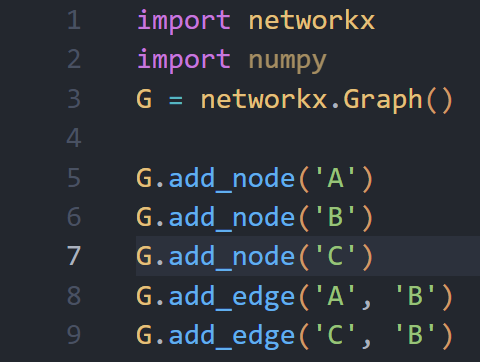
\includegraphics[width=8cm]{images/add_nodes_add_edges.png}\\
        The above code does the following: it imports the Networkx package for us to use, creates a 'graph' object called G, creates nodes A, B, C, then adds two edges between A and B and B and C.\\
        However that is too cumbersome for normal use so the Networkx package provides functions such as:
        \begin{verbatim}networkx.complete_graph(5)\end{verbatim}
        to generate a complete graph with 5 nodes in one line, but we still have very fine control of the graph as in the first example.
        \subsection{Creating Random Graphs}
        To create a random graph on a piece of paper it is quite simple: Select $N$ nodes to add to the graph and $p$ probability, draw $N$ nodes on the paper, then go through every possible pair of nodes in the graph and draw an edge between them if when picking a random real number from [0,1] it is less than $p$. Networkx implements a function \verb|networkx.gnp_random_graph| to create a random graph using the following code:\\
        \begin{figure}[H]
            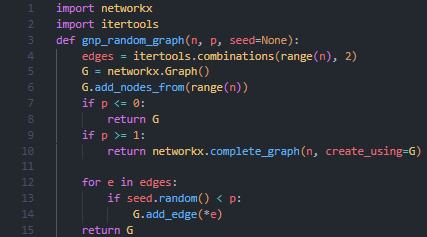
\includegraphics[width=8cm]{images/CreatingRandomGraphs.png}
            \caption{The Random Graph Function}
            \label{fig:RandomGraph1}
        \end{figure}
        Let us explain, the function takes $n$ (The total number of nodes) and $p$ (The probability of drawing an edge between a pair of nodes) as parameters. The \verb|itertools.combinations(range(n),2)| creates s list of every combination of 2 numbers up to $n$ i.e. (0,1), (0,2), (1,2) and so on, then to graph $G$ we add $n$ nodes, if $p = 0$ then there are 0 edges in the graph, so it stays empty and if $p =1$ then every node is attached to every other node, so it becomes a complete graph, if neither of those are true then we loop through all the possible combinations of nodes and choose a random number from $[0,1]$ and if that is less than $p$ we add an edge between those nodes.
        \subsection{Creating Barabasi-Albert Graphs}
        First let us describe how to create Barabasi-Albert Graphs on a piece of paper. To create a Barabasi-Albert Graph we must first start with a "seed" graph (An already drawn graph that we will grow using the Barabasi-Albert Model) then we will define two more parameters $n$ for the total number of nodes we want this new graph to have and $m$ the number of edges we will add each iteration of the model. The algorithm works in the following way: take your "seed" graph and assign each node on the graph a probability $p$ according to its degree $k$ using the formula $p(k_{i}) = \frac{k_{i}}{\sum_{j} {k_{j}}}$ we then randomly select $m$ unique nodes according to the probabilities calculated (this can be done by label each node 1 to n then write on a piece of paper that label for each node, then fold the paper a number of times proportional to its probability for example folding 0.2 twice but 0.2 five times then randomly choosing the papers), add 1 new node to the graph and draw an edge from this new node to each of the randomly pre-existing nodes, repeat this until we have $n$ nodes on the graph.\\
        As Barabasi-Albert graphs are the main focus of this project we will now show how they are created in networkx. 
        \begin{figure}[H]
            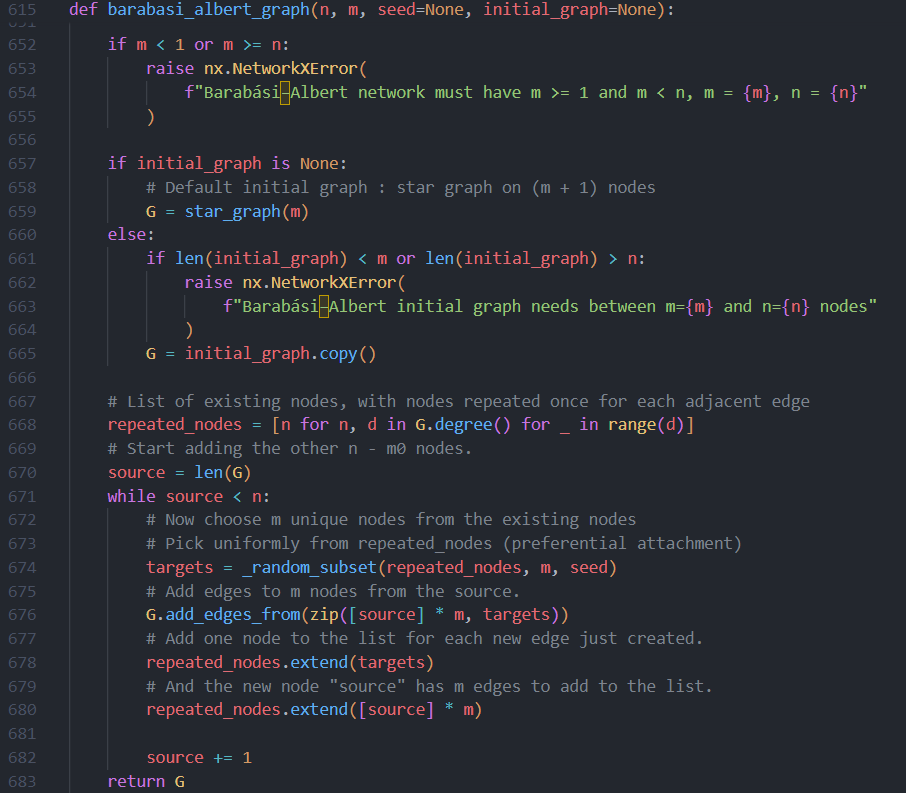
\includegraphics[width=12cm]{images/BARABASI_FUNC.png}
            \caption{The Barabasi-Albert Graph Function}
            \label{fig:Barabasi-Albert function1}
        \end{figure}
        This is the Barabási-Albert function from Networkx. It takes 4 parameters, $n$,$m$, \verb|seed|, and \verb|initial_graph|. $n$ and $m$ are simply the same as explained above, \verb|seed| is for the random functions later, so we can control the behaviour,  \verb|initial_graph| is where we input our 'seed graph' for the model to build on (If no graph is provided then it uses a Star graph with $(m+1)$ nodes). The function then creates a list of nodes: \verb|repeated_nodes| where each node is repeated equal to its degree (A node with degree $5$ is repeated 5 times) then takes random samples from this list to create the preferential attachment then finally returns the Barabási-Albert graph. 
        
        \subsection{Gaining Information From Graphs}
        Methods in networkx allow us to extract key information from the graph objects such as \verb|G.number_of_edges| which returns the number of edges that are contained in graph $G$ or \verb|networkx.all_neighbours(G,n)| which returns all the neighbours of node $n$ in graph $G$.
        \subsection{SIRD Model Code}
        The code can also be found in the dropbox link.

        \subsection{Acknowledgements}
        I would like to thank the following people for their assistance in this project: Firstly my girlfriend Jessica for ensuring I stay focused throughout and helping me proofread as well as emotional support, then I would like to thank Vince Kwasnica for being extremely helpful as my project supervisor and personal tutor given guidance and reigning in my project when I would nrealy run it off the tracks. And Finally I would like to thank the developers of Python, Networkx, Pandas and Scipy without their software the project would not have run as smoothly as it has and the maintainers of \LaTeX which proved extremely useful in the writing of this project.
\printbibliography
\end{document}